\documentclass[tikz,border=6pt]{standalone}
\usepackage{pgfplots}
\pgfplotsset{compat=1.18}
\definecolor{curveblue}{RGB}{37,99,235}
\definecolor{rootgreen}{RGB}{5,150,105}
\definecolor{vertexviolet}{RGB}{124,58,237}
\definecolor{axisgray}{RGB}{100,116,139}
\begin{document}
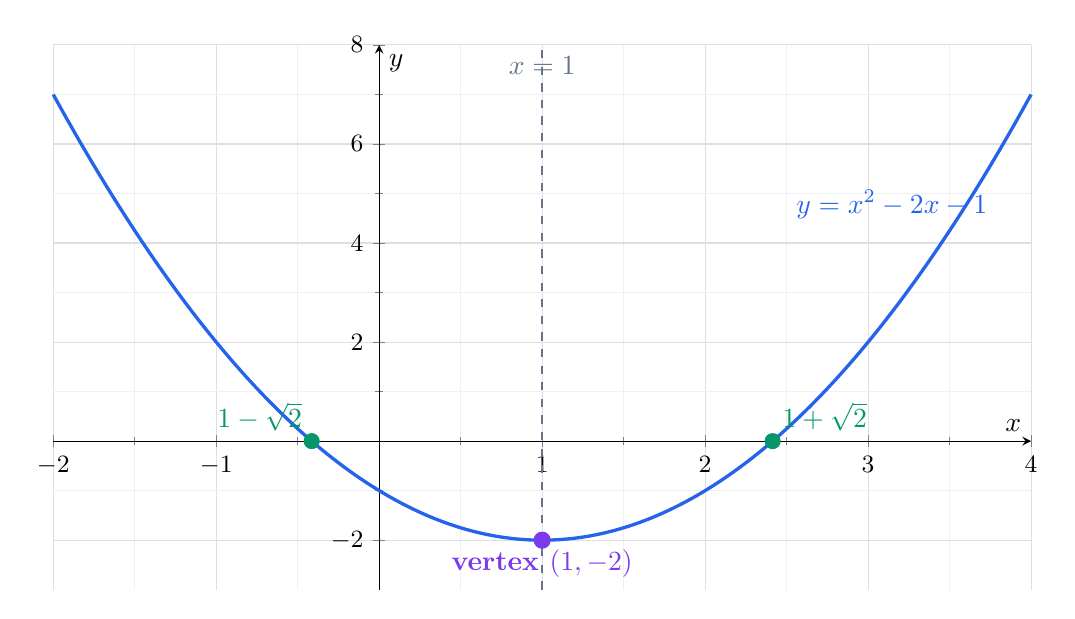
\begin{tikzpicture}
\begin{axis}[
  width=14cm,
  height=8.5cm,
  axis lines=middle,
  xlabel={$x$},
  ylabel={$y$},
  xmin=-2,
  xmax=4,
  ymin=-3,
  ymax=8,
  xtick={-2,-1,0,1,2,3,4},
  ytick={-2,0,2,4,6,8},
  grid=both,
  minor tick num=1,
  major grid style={draw=gray!25},
  minor grid style={draw=gray!12},
  tick label style={font=\small},
  label style={font=\bfseries},
  samples=240,
  clip=false,
]
\addplot[curveblue, very thick, domain=-2:4] {x^2 - 2*x - 1};
\addplot[axisgray, dashed, thick] coordinates {(1,-3) (1,8)};
\addplot[rootgreen, only marks, mark=*, mark size=2.7pt] coordinates {(1-sqrt(2),0) (1+sqrt(2),0)};
\addplot[vertexviolet, only marks, mark=*, mark size=2.9pt] coordinates {(1,-2)};
\node[anchor=south east, text=rootgreen, font=\bfseries] at (axis cs:{1-sqrt(2)},0) {$1-\sqrt2$};
\node[anchor=south west, text=rootgreen, font=\bfseries] at (axis cs:{1+sqrt(2)},0) {$1+\sqrt2$};
\node[anchor=north, text=vertexviolet, font=\bfseries] at (axis cs:1,-2) {vertex $(1,-2)$};
\node[anchor=south, text=axisgray, font=\bfseries] at (axis cs:1,7.2) {$x=1$};
\node[anchor=south west, text=curveblue, font=\bfseries] at (axis cs:2.5,4.3) {$y=x^2-2x-1$};
\end{axis}
\end{tikzpicture}
\end{document}
